\section{On Software Engineering}\label{sdp}
The sofware engineering lifecycle is host of several key process areas defined
for efficient organizations.

\subsection{Properties of Software}\label{software_props}
There are key attributes about software and documentation that make them 
intrinsically different from other fields of engineering. These areas 
distinguish software engineering from traditional engineering in a way that 
complicates the process for safety-critical organizations. These unique
differences (1) make it difficult to identify software as a ``product'' liable
under the strict liability standard and (2) discourage sound documentation and
commenting practices.

\subsubsection*{Material Costs}

There are no upfront material costs to begin software implementation. Generic,
over-the-shelf hardware like personal computers can be used to produce
tremendous feats in software engineering. In fact, Google, Inc. started by using
commodotity machines to build what is now one of the most ubiquitous search 
tools in computing \cite{Google}.

Because of this absence of material cost, it is easier for software engineers to
neglect to use certain precautions or care since there is no notion of immediate
damage of expensive equipment or loss due to injury. For example, an industrial
contractor may be dealing with expensive pieces of machinery when he installs
equipment for clients. This engineer would use extreme caution when working with
the machine, making repairs, or tooling with devices. He may even be working off
of very formal blueprints, instruction manuals, and installation documents. This
degree of formality is rarely seen in the software industry.

\subsubsection*{Product Replication}\label{software_product}
Since software is entirely digital, it is easily replicatable. This means that
there is no chance that a copy of software can ever be a diversion from the
original design. A bug found in any particular instance of a software program
will exhibit itself in all copies of that piece of software, including the
``original''.

\subsubsection*{Fast Turnaround}

More and more clients are demanding speed in implementation. Software developers
often deliver what is requested of them for immediate profit over long-term
gain. Stakeholders see no immediate benefit from quality documentation.

\subsubsection*{Testability}

Documentation is not testable. By their very nature, documentation and code
comments are open-ended artifacts with few restrictions or templates.

\subsection{The Software Development Process}
In order to build a quality software systems, many organizations follow a
formal, methodological approach to the development process. This process is
described in general below, but more specifically in \cite{Royce1970},
\cite{Boehm1986}, \cite{CMM11}, and \cite{Kehoe1996}.

\subsubsection{Waterfall Model}\label{waterfall}

\begin{figure}[t]
\begin{center}
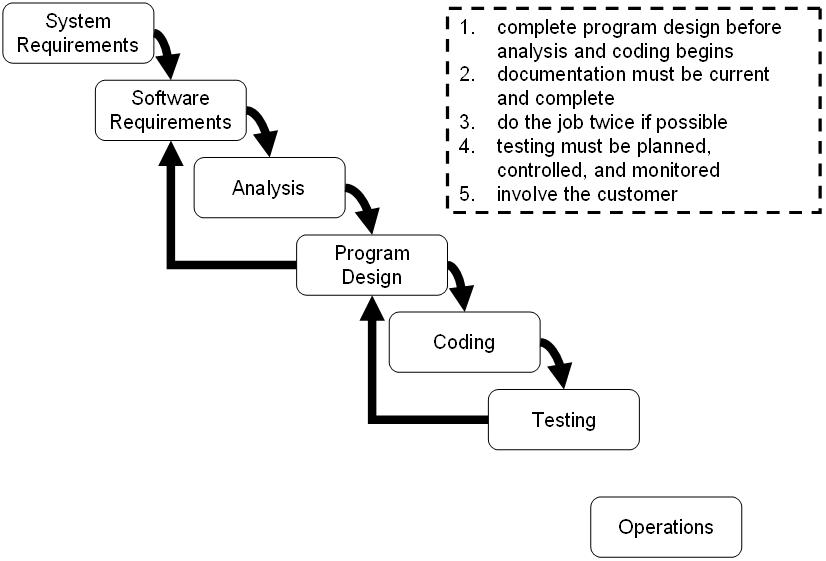
\includegraphics[scale=0.66]{images/waterfall.jpg}
\end{center}
\caption{Waterfall Model of the Software Process}
\label{fig:waterfall}
\end{figure}

The original treatment of the waterfall model appears in \cite{Royce1970} and
describes a specification-driven approach to software development. Figure
\ref{fig:waterfall} shows different phases that flow steadily downwards (like a
waterfall). The model stresses a sequential occurence of events in software
development, but also includes an iterative treatement to account for the
evolving software development process. For more information on the waterfall
model, see \cite{Royce1970}.

\subsubsection{Spiral Model}\label{spiral}

\begin{figure}[t]
\begin{narrow}{-1.5in}{-1.5in}
\begin{center}
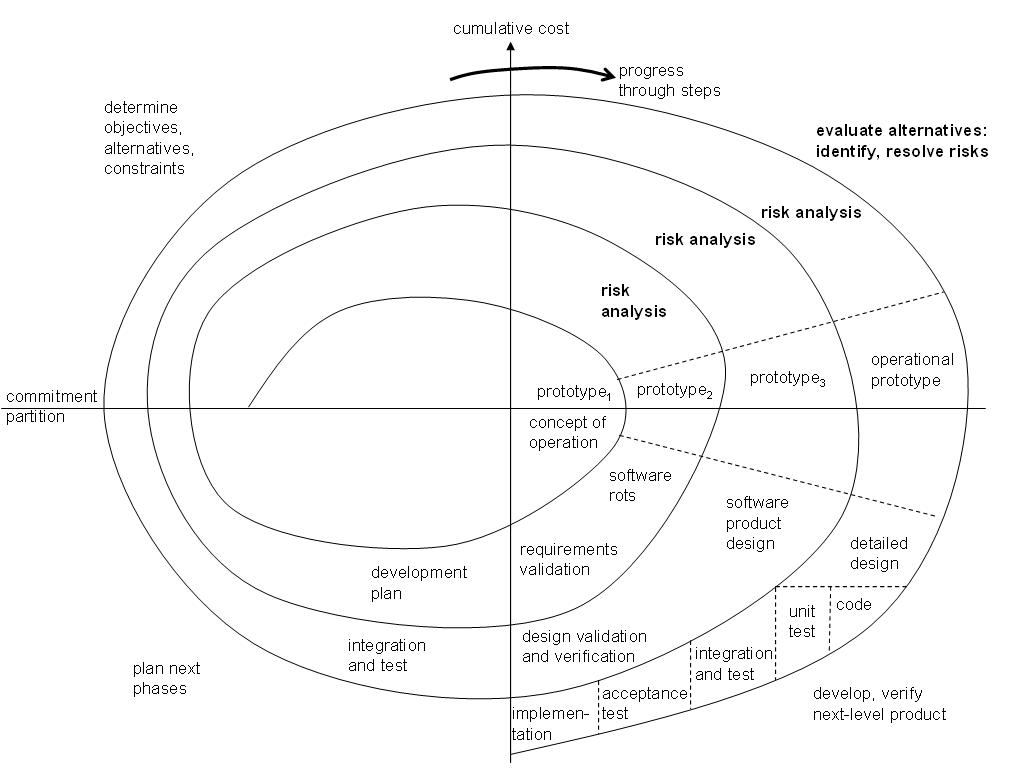
\includegraphics[scale=0.66]{images/spiral.jpg}
\end{center}
\end{narrow}
\caption{Spiral Model of the Software Process}
\label{fig:spiral}
\end{figure}

The spiral model, as described in \cite{Boehm1986}, builds on refinements made
to the waterfall model. Boehm explains that the sofware process as an iteration
of four phases of activity which can be retrofitted to particularize to a
variety of methods and approaches. As illustrated in Figure \ref{fig:spiral},
the radial dimension represents the cumulative osts incurred in accomplishing
the steps to date while the angular dimension represents the progress made in
completing each spiral.

Notice that each rotation around the spiral begins with objectives,
consideration of alternatives, and the constraints on the system so (cost,
schedule, interface, etc.). According to Boehm's model, software developers
should take risks into consideration and these considerations should be
documented. For more information on the spiral model, refer to \cite{Boehm1986}.
